\documentclass[aspectratio=169]{ISAE-Beamer}
\usepackage{amsmath,amssymb,amsthm}
\usepackage{bm}
\usepackage{graphicx}
\usepackage{diffcoeff}
\usepackage{dsfont}
\usepackage{mathrsfs}

\usepackage{multimedia}

\usepackage[backend=bibtex]{biblatex}

\graphicspath{{./Figures/}}

\bibliography{bib_pres_sxs}

\DeclareMathOperator{\Tr}{Tr}
\DeclareMathOperator*{\grad}{grad}
\DeclareMathOperator*{\Grad}{Grad}
\DeclareMathOperator*{\Div}{Div}
\renewcommand{\div}{\operatorname{div}}
\DeclareMathOperator*{\Hess}{Hess}

\DeclareMathOperator*{\argmax}{arg\,max}
\DeclareMathOperator*{\argmin}{arg\,min}

\def\onedot{$\mathsurround0pt\ldotp$}
\def\cddot{% two dots stacked vertically
	\mathbin{\vcenter{\baselineskip.67ex
			\hbox{\onedot}\hbox{\onedot}}%
}}

\makeatletter \renewcommand\d[1]{\ensuremath{%
		\;\mathrm{d}#1\@ifnextchar\d{\!}{}}}
\makeatother

\title[SXS Presentation]{Port-Hamiltonian modeling and control of  flexible structures.}

\institute[ISAE]
{\inst{1}ISAE-SUPAERO, Toulouse}

\author[Andrea Brugnoli]{Andrea Brugnoli\inst{1}}

\date[Pres SXS, 27/09/19]{September, the 27th, 2019}

%\thanks{}

\begin{document}

\maketitle

\begin{frame}{Outline}

\tableofcontents

\end{frame}

\section{PHD in theory and practice}

\begin{frame}{About me}
\textbf{Formation:}
\begin{itemize}
	\item High school diploma in Humanities, \textbf{Vérone};
	\item Bachelor in Mechanical Engineering, Politecnico di Milano, \textbf{Milan};
	\item Master of science in Space Engineering, Politecnico di Milano, \textbf{Milan};
	\item Double Degree Politecnico/Isae-SUPAERO, \textbf{Toulouse};
	\item Research Master in Automatic Control, Supélec, \textbf{Paris/Toulouse};
\end{itemize}
\centering
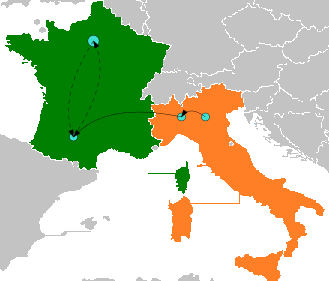
\includegraphics[height=0.4\textheight]{trip.png}
\end{frame}

\begin{frame}{PHD title and purposes}

\begin{block}{PHD title}
	Modeling and control by the Port-Hamiltonian formalism of 2D flexible structures with varying boundary conditions.
\end{block}
\begin{block}{Supervisors}
	Daniel Alazard \hspace{1.5cm} Valerie Budinger 
	\hspace{1.5cm}
	Denis Matignon
\end{block}
\begin{block}{Fundings}
	This work is funded by ISAE-SUPAERO.
\end{block} 

\begin{block}{Objectives}
	The knowledge of boundary conditions is mandatory for building models in Patran/Nastran (an a priori knowledge of overall system is required).  The pH framework on the contrary is highly modular and allow building a complex system form its subcomponents. Moreover, we aim to examine performance specifications in the PH formalism.
\end{block}
\end{frame}

\begin{frame}{What about the PHD reality}
	
\only<1>{\centering{\huge Impressions and ideas?}} 
\only<2>{My personal vision of PHD after two years:
	\begin{itemize}
		\item Less remunerate (but not always) than an engineer position but greater freedom (and intellectual gratification);
		\item Freedom also implies working on your own for the majority of time. However collaborations, meetings, presentations, social networking are also of crucial importance;
		\item Motivation, autonomy, perseverance are necessary conditions. Curiosity and willingness to learn by trials and errors are the driving force;
		\item A worldwide experience: researchers exchange towards frontiers and continents;
		\item Very enriching under a personal and intellectual point of view;
	\end{itemize}	
}
\end{frame}

\begin{frame}{A purely intellectual static activity?}
\begin{columns}
	\begin{column}{0.5\textwidth}
		Trips: conferences, meetings, schools
		\begin{itemize}
			\item Winter school in Paris, Sup\'elec;
			\item Spring school and project meeting in Wuppertal;
			\item International mobility to Brasil, at ITA;
			\item Conference at Oaxaca, CPDE-CDPS;
		\end{itemize}
	Upcoming trips:
	\begin{itemize}
		\item Project meeting in Besançon;
		\item CDC conference in Nice;
		\item IFAC World Congress in Berlin;
	\end{itemize}
	\end{column}
	\begin{column}{0.5\textwidth}
		\centering
		\includegraphics[height=0.8\textheight]{world_trip.eps}
	\end{column}
\end{columns}
\end{frame}

\section{Port Hamiltonian systems}

\begin{frame}{What does that mean?}
	The port-Hamiltonian formalism (Maschke, van der Schaft, 1992) brings together:
	\begin{itemize}
		\item Hamiltonian mechanics;
		\item Port-based modeling approach (bond-graph)
		\begin{itemize}
		\item Different domains (mechanical, electrical, hydraulic, thermal);
		\item Energy is the lingua franca;
		\item Complex systems are written as a composition of ideal components:
		energy-storage, energy-dissipation, energy-routing, etc; 
		\end{itemize}
	\item Passive systems and control theory.
	\end{itemize}
	
\end{frame}

\subsection{Finite dimensional pH systems}

\begin{frame}{From Lagrangian to Hamiltonian mechanics}
Lagrangian function: $L(q, \dot{q}, t) = \frac{1}{2} \dot{q}^T M(q) \dot{q} - V(q)$. \\
Define the generalize momenta as 
\[ p := \diffp{L}{\dot{q}}.
\]
The Hamiltonian is obtained by application of the Legendre transform
\[ H = p^T\dot{q} - L(q, \dot{q}, t).
\]
This new quantity depends only on $(q, p)$. Notice that 
\[
\diffp{H}{q} = -\diffp{L}{q}, \qquad \diffp{H}{p} = \dot{q} 
\]
\end{frame}

\begin{frame}

The Lagrange equation of motion for \only<1>{\textcolor{blue}{conservative systems}}\only<2>{\textcolor{blue}{dissipative systems $D = \frac{1}{2} r ||\dot{q}||^2$}}\only<3->{\textcolor{blue}{open dissipative systems $D = \frac{1}{2} r ||\dot{q}||^2$}}
\[
\diff{}{t}\diffp{L}{\dot{q}} - \diffp{L}{q} \only<2->{ + \textcolor{blue}{\diffp{D}{\dot{q}}}} = \only<1-2>{\textcolor{blue}{0}} \only<3->{\textcolor{blue}{u}} 
\]
can now be recast using the Hamiltonian
\[\diff{}{t}
\begin{bmatrix}
p \\ q \\
\end{bmatrix} = 
\begin{bmatrix}
\only<1>{0} \only<2->{\textcolor{blue}{-r}} & -1 \\ 
1 & 0 \\
\end{bmatrix}
\begin{bmatrix}
\partial_p{H} \\ 
\partial_q{H} \\
\end{bmatrix} \only<3->{+ 
	\begin{bmatrix}
	1 \\ 0 \\
	\end{bmatrix} \textcolor{blue}{u}
}
\]
If the energy rate is computed
\[ \dot{H} = \dot{p}^T \partial_p{H} + \dot{q}^T \partial_q{H} = \only<1>{\textcolor{blue}{0}} \only<2->{\textcolor{blue}{-r ||\partial_p(H)||^2}} \only<3->{\textcolor{blue}{ + u^T y}} 
\]
\only<3>{The output is chosen to be the energy conjugated variable to the input $y=\partial_p{H}$.}
\end{frame}

\begin{frame}{Finite-dimensional port-Hamiltonian systems}
General structure of an open Hamiltonian system with dissipation
\begin{align*}
\diff{}{t}
\begin{bmatrix}
p \\ q \\
\end{bmatrix} &= 
\begin{bmatrix}
-r & -1 \\ 
1 & 0 \\
\end{bmatrix}
\begin{bmatrix}
\partial_p{H} \\ 
\partial_q{H} \\
\end{bmatrix}+ 
\begin{bmatrix}
1 \\ 0 \\
\end{bmatrix} u \\
y &= \begin{bmatrix}
1 & 0 \\
\end{bmatrix} \begin{bmatrix}
\partial_p{H} \\ 
\partial_q{H} \\
\end{bmatrix}
\end{align*}
This system are also called port-Hamiltonian systems as the communicate to the outer world through ports.
\end{frame}



\begin{frame}{Finite-dimensional port-Hamiltonian systems}

\begin{columns}[T]
\begin{column}{0.45 \textwidth}
\begin{block}{Non linear finite dimensional pH system}
The Hamiltonian is a generic function of the state $H(x)$
	\begin{align*}
	\dot{x} &= (J - R) \partial_x{H} + B u \\
	y &= B^T \partial_x{H}
	\end{align*}
\end{block}
\end{column}
\begin{column}{0.45 \textwidth}
\begin{block}{Linear finite dimensional pH system}
	The Hamiltonian is a quadratic function of the energy variables $H = \frac{1}{2} x^T Q x$
	\begin{align*}
	\dot{x} &= (J - R) Q x + B u \\
	y &= B^T Q x
	\end{align*}
\end{block}
\end{column}
\end{columns}
\vspace{1mm}
Nomenclature:
\begin{itemize}
	\item $x$ energy variables; \\
	\item $e:=\partial_x{H}$ co-energy variables; \\
	\item $J = -J^T$ interconnection matrix (skew symmetric); \\
	\item $R = R^T, \, R \succeq 0$ dissipation matrix (symmetric positive semi-definite); \\
\end{itemize}

\end{frame}

\begin{frame}{Interconnection of pH systems}
If the interconnection is power-preserving then the resulting system is again pH.
\begin{columns}[T]
	\begin{column}{.25\textwidth}
		\begin{block}{Individual systems}
			System 1:
			\begin{align*}
			\dot{x}_1 &= J_1 \ \partial_{x_1}{H_1} + B_1 u_1 \\
			y_1 &= B_1^T \ \partial_{x_1}{H_1}
			\end{align*}
			System 2:
			\begin{align*}
			\dot{x}_2 &= J_2 \ \partial_{x_2}{H_2} + B_2 u_2 \\
			y_2 &= B_2^T \ \partial_{x_2}{H_2}
			\end{align*}	
		\end{block}
	\end{column}
\only<2>{
\begin{column}{.20\textwidth}
\vspace{1cm}
Gyrator interconnection
\begin{align*}
	u_1 &= y_2 + u_e \\
	u_2 &= -y_1
\end{align*}
\end{column}
\begin{column}{.55\textwidth}	
	\begin{block}{Coupled system}
	$H(x_1, x_2) = H_1(x_1) + H_2(x_2)$
		\begin{align*}
		\diff{}{t}
		\begin{bmatrix}
		x_1 \\ x_2 \\
		\end{bmatrix} &= 
		\begin{bmatrix}
		J_1 & B_1 B_2^T \\ 
		- B_2 B_1^T & J_2 \\
		\end{bmatrix}
		\begin{bmatrix}
		\partial_{x_1}{H} \\ 
		\partial_{x_2}{H} \\
		\end{bmatrix}+ 
		\begin{bmatrix}
		B_1 \\ 0 \\
		\end{bmatrix} u_e \\
		y_e &= \begin{bmatrix}
		B_1^T & 0 \\
		\end{bmatrix} \begin{bmatrix}
		\partial_{x_1}{H} \\ 
		\partial_{x_2}{H} \\
		\end{bmatrix}
		\end{align*}	
	\end{block}
\end{column}
}
\only<3>{
	\begin{column}{.20\textwidth}
		\vspace{1cm}
		Transformer interconnection
		\begin{align*}
		u_1 &= - u_2 + u_e \\
		y_2 &= y_1
		\end{align*}
	\end{column}
	\begin{column}{.55\textwidth}	
		\begin{block}{Coupled system}
			$H(x_1, x_2) = H_1(x_1) + H_2(x_2)$
			\begin{align*}
			\diff{}{t}
			\begin{bmatrix}
			x_1 \\ x_2 \\ 0 \\
			\end{bmatrix} &= 
			\begin{bmatrix}
			J_1 & 0 & -B_1 \\ 
			0 & J_2 & B_2 \\
			B_1^T & - B_2^T & 0 \\
			\end{bmatrix}
			\begin{bmatrix}
			\partial_{x_1}{H} \\ 
			\partial_{x_2}{H} \\
			\lambda \\
			\end{bmatrix}+ 
			\begin{bmatrix}
			B_1 \\ 0 \\ 0 \\
			\end{bmatrix} u_e \\
			y_e &= \begin{bmatrix}
			B_1^T & 0 & 0 \\
			\end{bmatrix} \begin{bmatrix}
			\partial_{x_1}{H} \\ 
			\partial_{x_2}{H} \\
			\lambda \\
			\end{bmatrix}
			\end{align*}
			This is a differential-algebraic system (pHDAE)	
		\end{block}
	\end{column}
}
\end{columns}

\end{frame}

\subsection{Infinite dimensional pH systems}

\begin{frame}{Infinite dimensional systems}
Even PDE models can be put in Hamiltonian form \footfullcite{Olver}. Consider the Euler-Bernoulli beam model
\begin{equation*}
\rho A(z) \diffp[2]{w}{t} + \diffp[2]{}{z} \left(EI(z) \diffp[2]{w}{z} \right) =0 \quad z \in [0, L] \quad + \text{Boundary conditions}
\end{equation*}
Total energy of the system
\begin{equation*}
H = \frac{1}{2} \int_{0}^{L} \rho A(z) \left(\diffp{w}{t} \right)^2 +  EI(z) \left(\diffp[2]{w}{z} \right)^2 \d{z}
\end{equation*}
Select as energy variables $x_1 = \rho A(x) \diffp{w}{t}, \; x_2 = \diffp[2]{w}{z}$. \begin{equation*}
H = \frac{1}{2} \int_{0}^{L} \frac{1}{\rho A(z)} x_1^2 +  EI(x) x_2^2 \d{z}
\end{equation*}
\end{frame}

\begin{frame}{PDE and pH systems}
The energy is no more a function but a functional. The co-energy variables are given by the variational derivative with respect to the state
\begin{equation*}
e_1 := \diffd{H}{x_1} = \diffp{w}{t}, \qquad e_2 := \diffd{H}{x_2} = EI(z) \diffp[2]{w}{x}
\end{equation*}
The Euler Bernoulli beam model is then rewritten as
\begin{equation*}
\diffp{}{t} \begin{bmatrix}
x_1 \\ x_2 \\
\end{bmatrix} = 
\underbrace{\begin{bmatrix}
0 & -\diffp[2]{}{z} \\
\diffp[2]{}{z} & 0 \\
\end{bmatrix}}_{\mathcal{J}}
\begin{bmatrix}
e_1 \\
e_2 \\
\end{bmatrix}
\end{equation*}
The operator $\mathcal{J}$ is formally skew-adjoint (infinite dimensional extension of the skew-symmetric property of a matrix). That means that for homogeneous boundary conditions
\[
<x, \mathcal{J} y >_{\mathcal{H}} \underbrace{=}_{\text{i.b.p.}} <- \mathcal{J} x, y >_{\mathcal{H}}
\]
where $\mathcal{H}$ is an Hilbert space.
\end{frame}

\begin{frame}{Energy rate}
From the energy balance the boundary variables are readily found
\begin{equation*}
	\dot{H} = \int_{0}^L \diffp{x}{t}^T \diffd{H}{x} \d{x} = \int_{0}^L e^T \mathcal{J} e \d{x} \underbrace{=}_{\text{i.b.p.}} \left(e_2 \diffp{e_1}{x} - e_1 \diffp{e_2}{x}\right)\bigg\rvert_0^L.
\end{equation*}
The energy rate equals a scalar product of the standard boundary condition:
\begin{itemize}
\item $e_1\vert_{\partial\Omega} = \partial_t w\vert_{\partial\Omega}$: vertical velocities;
\item $\partial_{x} e_1\vert_{\partial\Omega} = \partial_{xt} w\vert_{\partial\Omega}$: vertical angular velocities;
\item $e_2\vert_{\partial\Omega} = EI \partial_{xx} w\vert_{\partial\Omega}$: bending momenta;
\item $\partial_{x} e_2\vert_{\partial\Omega} =\partial_x(EI \partial_{xx}w)\vert_{\partial\Omega}$: shear forces;
\end{itemize}
Thanks to this structure important properties of pH boundary control system can be easily checked \footfullcite{LeGorrec2005}.
\end{frame}

\begin{frame}{Infinite dimensional pH systems}
\begin{block}{\only<1>{General}\only<2>{Linear} infinite dimensional pH system}
\begin{equation*}
\begin{cases}
\displaystyle \diffp{x}{t}(z, t) &= \mathcal{J} \only<1>{\diffd{H}{x}} \only<2>{\mathcal{Q} x} + B \textcolor{red}{u(z, t)}, \\
\displaystyle \textcolor{red}{y(z, t)} &= B^* \diffd{H}{x}.
\end{cases}
\end{equation*}
With boundary conditions
\[\textcolor{blue}{u_\partial} = \mathcal{B} \diffd{H}{x}, \quad \textcolor{blue}{y_\partial} = \mathcal{C} \diffd{H}{x} \]
Energy rate: $\dot{H} = \displaystyle \textcolor{blue}{u_\partial^T y_\partial} +  \int_{\Omega} \textcolor{red}{u(z, t) y(z, t)} \d{\Omega}$
\begin{itemize}
	\item $x$ energy variables, $e = \delta_x H = \only<2>{\mathcal{Q} x}$: co-energy variables;
	\item $\mathcal{J}$: skew-symmetric differential operator;
	\item $\mathcal{B}, \mathcal{C}$: boundary operator;
	\item $u, y, B$: distributed input, output and control operator;
\end{itemize}
\end{block}
\end{frame}

\begin{frame}{Linear elasticity in PH form}
\only<1-3>{The general PDE for the elastodynamics (linear elasticity) reads
\begin{equation*}
	\rho \diffp[2]{u}{t} - \Div\left(\mathbb{D} \Grad(u)\right) = f.
\end{equation*}
}
\only<1>{
\begin{itemize}
	\item $\rho$ mass density, $\mathbb{D}$ stiffness tensor;
	\item $u$ displacement vector;
	\item $\Div$ divergence of a tensor, $\Grad =\frac{1}{2} \left[\nabla + \nabla^T\right]$ symmetric gradient of a vector;
	\item $f$ Body force;
\end{itemize}
Total energy: $\displaystyle H = \frac{1}{2} \int_{\Omega} \left\{\rho \left(\diffp{u}{t}\right)^2 + \Sigma \cddot \epsilon \right\} \d{\Omega}$,
\begin{itemize}
\item $\epsilon = \Grad(u)$, infinitesimal strain tensor, \\
\item $\Sigma = \mathbb{D} \ \varepsilon$, Cauchy stress tensor. 
\end{itemize}
}
\only<2>{To get a pH representation the energy variable have to selected:
	\begin{align*}
		x_1 &= \rho \diffp{u}{t}, \quad \text{Linear Momentum}, \\
		x_2 &= \Grad(u) = \varepsilon, \quad \text{Strain tensor}.
	\end{align*}
The corresponding co-energy are then retrieved
\begin{align*}
e_1 &= \diffd{H}{x_1} =  \diffp{u}{t}, \quad \text{Linear velocity}, \\
e_2 &= \diffd{H}{x_2} = \Sigma, \quad \text{Stress tensor}.
\end{align*}
}
	\only<3->{
	The pH system representing the elastodynamics equation becomes 
	\begin{equation*}
	\diffp{}{t}
	\begin{bmatrix}
	x_1 \\ x_2 \\
	\end{bmatrix} = 
	\begin{bmatrix}
	0 & \Div \\ \Grad & 0 \\
	\end{bmatrix}
	\begin{bmatrix}
	\rho^{-1} & 0 \\ 0 & \mathbb{D} \\
	\end{bmatrix}
	\begin{bmatrix}
	x_1 \\ x_2 \\
	\end{bmatrix} + 
	\begin{bmatrix}
	1 \\ 0 \\
	\end{bmatrix} f 
	\end{equation*}
	Together with appropriate boundary condition. \\ \vspace{1cm}
}
	\only<4>{\centering{Neumann control}
	\begin{align*}
	\textcolor{blue}{u_\partial} &= \Sigma \cdot n   \quad \text{on } \partial\Omega, \\
	\textcolor{red}{y_\partial} &= \diffp{u}{t}  \quad \text{on } \partial\Omega
	\end{align*}	
	}
	\only<5>{\centering{Dirichlet control}
	\begin{align*}
	\textcolor{blue}{u_\partial} &= \diffp{u}{t} \quad \text{on } \partial\Omega \\
	\textcolor{red}{y_\partial} &= \Sigma \cdot n \quad \text{on } \partial\Omega 
	\end{align*}	
	}
	\only<6>{\centering{Mixed control ($\partial\Omega = \Gamma_D \cup \Gamma_N$)}
	\begin{equation*}
	\begin{aligned}
	\textcolor{blue}{u_\partial} &= \partial_t u \quad \text{on } \Gamma_D, \\
	\textcolor{red}{y_\partial} &= \Sigma \cdot n \quad \text{on } \Gamma_D
	\end{aligned} \qquad 
	\begin{aligned}
	\textcolor{blue}{u_\partial} &= \Sigma \cdot n \quad \text{on } \Gamma_N \\
	\textcolor{red}{y_\partial} &= \partial_t u \quad \text{on } \Gamma_N
	\end{aligned}
	\end{equation*}
	}
\end{frame}

\begin{frame}{Some mechanical models}
\begin{columns}
	\begin{column}{.5\textwidth}
	Euler Bernoulli beam
	\begin{equation*}
	\mathcal{J}_{\text{EB}} = 
	\begin{bmatrix}
	0 & -\diffp[2]{}{z} \\
	\diffp[2]{}{z} & 0 \\
	\end{bmatrix}
	\end{equation*}
	\end{column}
	\begin{column}{.5\textwidth}
	Kirchhoff plate
	\begin{equation*}
	\mathcal{J}_{\text{K}} = 
	\begin{bmatrix}
	0 & -\div\Div \\ \Grad\grad & 0 \\
	\end{bmatrix}
	\end{equation*}
	\end{column}
\end{columns}
\vspace{1cm}
\begin{columns}
	\begin{column}{.5\textwidth}
	Timoshenko beam
	\begin{equation*}
	\mathcal{J}_{\text{T}} = 
	\begin{bmatrix}
	0 &  0 & 0 & \diffp{}{z} \\
	0 & 0 & \diffp{}{z} & 1  \\
	0 & \diffp{}{z} & 0 & 0  \\
	\diffp{}{z} & -1 & 0 & 0 \\
	\end{bmatrix}
	\end{equation*}
	\end{column}
	\begin{column}{.5\textwidth}
	Mindlin-Reissner plate
	\begin{equation*}
	\mathcal{J}_{\text{M}} = 
	\begin{bmatrix}
	0 &  0 & 0 & \div \\
	0 & 0 & \Div & \mathds{1} \\
	0 & \Grad & 0 & 0  \\
	\grad & -\mathds{1} & 0 & 0 \\
	\end{bmatrix}
	\end{equation*}
	\end{column}
\end{columns}
\vspace{1cm}
This model are obtained by imposing some assumptions on the displacement field from general 3D elasticity.
\end{frame}


\section{Numerics for pH system}

\begin{frame}{How to discretize pH systems?}
\begin{columns}[T]
	\setlength{\abovedisplayskip}{1pt}
	\setlength{\belowdisplayskip}{1pt}
	\begin{column}{.4\textwidth}
	\begin{block}{Infinite dimensional pHs}
		PDE:
		\begin{align*}
		\dot{x}(z, t) &= \mathcal{J} \delta_x {H} + B \textcolor{red}{u(z, t)}, \\
		\textcolor{red}{y(z, t)} &= B^* \delta_x {H}.
		\end{align*}
		Boundary conditions: 
		\[\textcolor{blue}{u_\partial} = \mathcal{B}\ \delta_x {H}, \quad \textcolor{blue}{y_\partial} = \mathcal{C}\ \delta_x {H} \]
		Power balance: 
		\[ \dot{H} = \displaystyle \textcolor{blue}{u_\partial^T y_\partial} +  \int_{\Omega} \textcolor{red}{u(z, t) y(z, t)} \d{\Omega}
		\]
	\end{block}
\end{column}
\begin{column}{.4\textwidth}
	\begin{block}{Finite dimensional pHs}
		ODE:
		\begin{align*}
		\dot{x} &= J \partial_x {H} + B_d \textcolor{red}{u_d} + B_\partial \textcolor{blue}{u_\partial}, \\
		\textcolor{red}{y_d} &= B_d^T \partial_x {H}, \\
		\textcolor{blue}{y_\partial} &= B_\partial^T \partial_x {H}
		\end{align*}
		Power balance: 
		\[ \dot{H} = \textcolor{blue}{u_\partial^T y_\partial} +  \textcolor{red}{u_d^T y_d}
		\]
	\end{block}
\end{column}
\end{columns}
\begin{exampleblock}{Available methods}
\begin{itemize}
	\item Spectral methods (Moulla 2012);
	\item Finite differences (Trenchant 2018);
	\item Finite elements based (Golo 2004, Kotyczka 2018, \textcolor{blue}{Cardoso-Riberio 2019});
\end{itemize}
\end{exampleblock}
\end{frame}

\begin{frame}{FEM for pHS }
A partitioned Finite Element method (PFEM) is our method of choice for its versatility:
\begin{itemize}
	\item Any geometrical dimension can be treated;
	\item Existent finite element libraries may be used;
	\item Easy to be implemented;
\end{itemize}
\end{frame}

\begin{frame}{General idea of PFEM}
General form of a pH system
\begin{equation*}
	\diffp{x}{t} = \mathcal{J} e, \qquad e = \diffd{H}{x}
\end{equation*}
In general it holds $\mathcal{J} = \sum_i \mathcal{J}_i$ (sum of skew-symmetric differential and algebraic operators). \\
\begin{block}{General procedure for PFEM}
\setlength{\abovedisplayskip}{1pt}
\setlength{\belowdisplayskip}{1pt}
\begin{enumerate}
\item Put the system into weak form:
\begin{equation*}
\left(v, \diffp{x}{t} \right)_{\Omega} = \left(v, \sum_i \mathcal{J}_i e \right)_{\Omega}.
\end{equation*}
\item Apply integration by part on each differential $\mathcal{J}_i$:
\begin{equation*}
\left(v, \sum_i \mathcal{J}_i e \right)_{\Omega} \overbrace{=}^{i.b.p.} j(v, e)_{\Omega} + b(v, u_\partial)_{\partial \Omega},
\end{equation*}
so that $j(v, e)_{\Omega}$ is a skew-symmetric bilinear form.
\item Discretization using a Galerkin method (same basis function for test, energy and co-energy variables)
\end{enumerate}
\end{block}
\end{frame}


\begin{frame}{Finite dimensional system}
Once all the steps are carried out, the following system is obtained
\begin{equation*}
	M \dot{x}_d = J e_d + B_d u_d.
\end{equation*}
The Hamiltonian still need to be discretized
\begin{equation*}
\dot{H}(x) = \int_{\Omega} \dot{x}^T \delta_x H \d{\Omega} = \int_{\Omega} \dot{x}^T e \d{\Omega}
\end{equation*}
If the approximated variable are introduced:
\begin{equation*}
\dot{H}_d(x_d) = \dot{x}_d^T \partial_{x_d} H_d = \dot{x}_d^T M e_d
\end{equation*}
Leading to: $e_d = M^{-1}\partial_{x_d} H_d$. 
Now taking $J_d = M^{-1} J M^{-1}$ a standard pH system is obtained
\begin{align*}
	\dot{x}_d &= J_d \partial_{x_d} H_d + B_d u_d, \\
	y_d &= B_d \partial_{x_d} H_d
\end{align*}
\end{frame}

\begin{frame}{Finite dimensional system (Linear case)}
If the system is linear the relation between energy and co-energy is trivial $e = \mathcal{Q} \alpha$. Assuming $Q$ coercive and symmetric (always verified for standard models), then the weak form may be rewritten as
\begin{equation*}
\left(v, \mathcal{Q}^{-1} \diffp{e}{t} \right)_{\Omega} = \left(v, \mathcal{J} e \right)_{\Omega}.
\end{equation*}
Applying the PFEM procedure it is obtained
\begin{align*}
M_d \dot{e}_d &= J_d e_d + B_d u_d, \\
y_d &= B_d e_d.
\end{align*}
This representation is also possible. When the problem is large inverting the mass matrix is unfeasible. The co-energy variables are even more meaningful than the energy ones.
\end{frame}

\begin{frame}[t]{The boundary term}
Different boundary terms arise from the integration by parts. \\ Consider the Euler Bernoulli beam in weak form:
\begin{align*}
\int_\Omega v^T \dot{x} \d\Omega &= \int_0^L \only<1>{-v_1 \diffp[2]{e_2}{z} + v_2 \diffp[2]{e_1}{z}} \only<2-3>{\textcolor{blue}{-v_1 \diffp[2]{e_2}{z}} + v_2 \diffp[2]{e_1}{z}} \only<4-5>{-v_1 \diffp[2]{e_2}{z} \textcolor{blue}{+v_2 \diffp[2]{e_1}{z}} } \d{x} \\
\only<3>{&= \int_0^L  \textcolor{blue}{-\diffp[2]{v_1}{z} e_2} + v_2 \diffp[2]{e_1}{z} \d{x} \textcolor{red}{- v_1 \diffp{e_2}{z}\bigg\vert_0^L + \diffp{v_1}{z} e_2 \bigg\vert_0^L} }
\only<5>{&= \int_0^L - v_1 \diffp[2]{e_2}{z} \textcolor{blue}{+ \diffp[2]{v_2}{z} e_1}   \d{x} \textcolor{red}{+ v_2 \diffp{e_1}{z}\bigg\vert_0^L + \diffp{v_2}{z} e_1 \bigg\vert_0^L} }
\end{align*}
\only<3>{
Control given by forces $\textcolor{red}{\diffp{e_2}{z}\vert_{\partial \Omega} = F\vert_{\partial \Omega}}$ and momenta $\textcolor{red}{e_2\vert_{\partial \Omega}=M\vert_{\partial \Omega}}$. \\ The uncontrolled system corresponds to the Free-Free case
\begin{figure}
	\includegraphics[width=0.18\textwidth]{EigenvectorsEB/FF_n1.eps} 
	\includegraphics[width=0.18\textwidth]{EigenvectorsEB/FF_n2.eps}
	\includegraphics[width=0.18\textwidth]{EigenvectorsEB/FF_n3.eps}  
	\includegraphics[width=0.18\textwidth]{EigenvectorsEB/FF_n4.eps} 
	\includegraphics[width=0.18\textwidth]{EigenvectorsEB/FF_n5.eps} 
\caption{Eigenvectors for the uncontrolled system}
\end{figure}
}
\only<5>{
	Control given by angular velocities $\textcolor{red}{\diffp{e_1}{z}\vert_{\partial \Omega} = \partial_{xt} w\vert_{\partial \Omega}}$ and linear velocities $\textcolor{red}{e_1\vert_{\partial \Omega}=\partial_{t} w\vert_{\partial \Omega}}$. \\ The uncontrolled system corresponds to the Clamped-Clamped case.
	\begin{figure}
		\includegraphics[width=0.18\textwidth]{EigenvectorsEB/CC_n1.eps} 
		\includegraphics[width=0.18\textwidth]{EigenvectorsEB/CC_n2.eps}
		\includegraphics[width=0.18\textwidth]{EigenvectorsEB/CC_n3.eps}  
		\includegraphics[width=0.18\textwidth]{EigenvectorsEB/CC_n4.eps} 
		\includegraphics[width=0.18\textwidth]{EigenvectorsEB/CC_n5.eps} 
		\caption{Eigenvectors for the uncontrolled system}
	\end{figure}
}
\end{frame}

\begin{frame}{Mixed boundary control}
If a system is controlled with two different kind of boundary input, the PFEM has to be adjusted. \\
\vspace{1cm}
Two possible methodology can be adopted:
\begin{itemize}
\item Domain decomposition and interconnection of two models with different inputs (not discussed here); \\
\item Lagrange multiplier; 
\end{itemize}

\end{frame}

\begin{frame}[t]{Lagrange multiplier}
The control input $u$ arising from the integration by parts is not known everywhere.\\
Lagrange multiplier must be introduced.

\begin{block}{Port Hamiltonian descriptor system}
	Generalization of the standard formulation. More general formulations exist. 
\begin{align*}
\begin{bmatrix}
\mathds{1} & 0 \\
0 & 0 \\
\end{bmatrix}\diff{}{t}
\begin{bmatrix}
x \\ \lambda\\
\end{bmatrix} &= 
\begin{bmatrix}
J & G \\
-G^T & 0 \\
\end{bmatrix}
\begin{bmatrix}
\partial_{x} H \\ \lambda \\
\end{bmatrix}
+ \begin{bmatrix}
B_x & 0 \\ 0 & B_\lambda \\
\end{bmatrix} \begin{bmatrix}
u_x \\ u_\lambda\\
\end{bmatrix}, \\
\begin{bmatrix}
y_x \\ y_\lambda\\
\end{bmatrix} &= \begin{bmatrix}
B_x^T & 0 \\ 0 & B_\lambda^T \\
\end{bmatrix} \begin{bmatrix}
\partial_{x} H \\ \lambda\\
\end{bmatrix}
\end{align*}
This formulation allow to consider mixed homogeneous and inhomogeneous boundary conditions and generic boundary control law.
\end{block}
\end{frame}

\begin{frame}{A simple application: eigenmodes computation}
Given a descriptor model the eigenvectors for arbitrary boundary condition may be computed.
\begin{figure}
	\includegraphics[width=0.19\textwidth]{EigenvectorsM/Eig_1.eps} 
	\includegraphics[width=0.19\textwidth]{EigenvectorsM/Eig_2.eps}
	\includegraphics[width=0.19\textwidth]{EigenvectorsM/Eig_3.eps}  
	\includegraphics[width=0.19\textwidth]{EigenvectorsM/Eig_4.eps} 
	\includegraphics[width=0.19\textwidth]{EigenvectorsM/Eig_5.eps}
	\includegraphics[width=0.19\textwidth]{EigenvectorsM/Eig_6.eps} 
	\includegraphics[width=0.19\textwidth]{EigenvectorsM/Eig_7.eps}
	\includegraphics[width=0.19\textwidth]{EigenvectorsM/Eig_8.eps}  
	\includegraphics[width=0.19\textwidth]{EigenvectorsM/Eig_9.eps} 
	\includegraphics[width=0.19\textwidth]{EigenvectorsM/Eig_10.eps}  
	\caption{Eigenvectors for the CCCF condition of the Mindlin plate by solving $Ev = j\omega Jv$}
\end{figure}
\end{frame}

\begin{frame}{Eliminating the Lagrange multipliers}
In structural dynamics applications  components are clamped on part of the boundary and free elsewhere (solar panels, robotic arms). However, the control is normally given either by distributed actuation, either by boundary forces and torques. \\

Consider a linear pHDAE system in co-energy variables
\begin{align*}
\begin{bmatrix}
M & 0 \\
0 & 0 \\
\end{bmatrix}\diff{}{t}
\begin{bmatrix}
e \\ \lambda\\
\end{bmatrix} &= 
\begin{bmatrix}
J & G \\
-G^T & 0 \\
\end{bmatrix}
\begin{bmatrix}
e \\ \lambda \\
\end{bmatrix}
+ \begin{bmatrix}
B  \\ 0 \\
\end{bmatrix}u, \\
y &= \begin{bmatrix}
B^T & 0 \\
\end{bmatrix} \begin{bmatrix}
e \\ \lambda\\
\end{bmatrix}
\end{align*}
Multiplying by the left annihilator of the constraint $G^\perp G = 0$ and applying the variable change $(G^\perp)^T \widehat{e} = e$, the constraints disappear
\begin{equation*}
\widehat{M} \ \dot{\widehat{e}} = \widehat{J} \widehat{e} + \widehat{B} u 
\end{equation*}

\end{frame}

\begin{frame}{Main research points}
	The numerical discretization of pHs is a very recent field. 
	\begin{itemize}
		\item Ongoing work on the optimal convergence rate for the wave equation;
		\item Electrodynamics and structural mechanics require further investigation\footfullcite{ArnoldElasDyn} \, \footfullcite{becache};  
	\end{itemize}
\end{frame}

\section{Control theory and pH system}

\begin{frame}{Damping assignment and control by interconnection\footfullcite{ORTEGAsurvey}}

\begin{block}{Energy shaping}
	The interconnection with a suitable controller allows to shape the energy, so that its minimum is located at a desired configuration $u = u_{\text{ES}} + v$:
	\begin{equation*}
	\begin{bmatrix}
	\dot{p} \\ \dot{q} \\
	\end{bmatrix} = 
	\begin{bmatrix}
	0 & -I \\ 
	I & 0 \\
	\end{bmatrix}
	\begin{bmatrix}
	\partial_p{H} \\ 
	\partial_q{H} \\
	\end{bmatrix}+ 
	\begin{bmatrix}
	G(q) \\ 0 \\
	\end{bmatrix} u 
	\quad \longrightarrow \quad
	\begin{bmatrix}
	\dot{p} \\ \dot{q} \\
	\end{bmatrix} = 
	\begin{bmatrix}
	0 & -J_1^T(q) \\ 
	J_1(q) & 0 \\
	\end{bmatrix}
	\begin{bmatrix}
	\partial_p{H_d} \\ 
	\partial_q{H_d} \\
	\end{bmatrix} + 
	\begin{bmatrix}
	G(q) \\ 0 \\
	\end{bmatrix} v
	\end{equation*}
\end{block}

\begin{exampleblock}{Damping Injection}
PH system are collocated: input and output are energy conjugated. The simple control law 
\[v= - K_{\text{DI}} G^T(q) \partial_p H_d(q, p) \]
 always inject damping into the system.
\end{exampleblock}
\end{frame}

\begin{frame}{Model Reduction}
\only<1>{
\begin{block}{Time domain methodologies}
	For non-linear pH system the Proper Orthogonal Decomposition is available. Given the optimization problem:
	\begin{equation*}
	P_* = \argmin_{\text{rank}(P)=r} \int_0^\infty ||(I - P)x(t)||^2 \d{t}, \qquad
	Q_* = \argmin_{\text{rank}(P)=r} \int_0^\infty ||(I - P)\partial_x H(x(t))||^2 \d{t}.
	\end{equation*}
	The reduction system is given by the Petrov-Galerkin projection using as subspaces $\mathcal{V}_r = \text{Ran}(P_*), \; \mathcal{W}_r = \text{Ran}(Q_*)$.
\end{block}
\begin{alertblock}{Frequency domain techniques}
\setlength{\abovedisplayskip}{1pt}
\setlength{\belowdisplayskip}{1pt}
One may use $\mathcal{H}_2/\mathcal{H}_\infty$ optimal subspaces. They try to match the full and reduced transfer functions
\begin{equation*}
G(s) = B^T (s Q^{-1} - (J-R))^{-1} B \qquad G_r(s) = B_r^T (s Q_r^{-1} - (J_r-R_r))^{-1} B_r
\end{equation*}
Krilov subspaces method (moment matching) can also be used and work fine for pHDAE.
\end{alertblock}
}
\only<2>{
\begin{figure}
	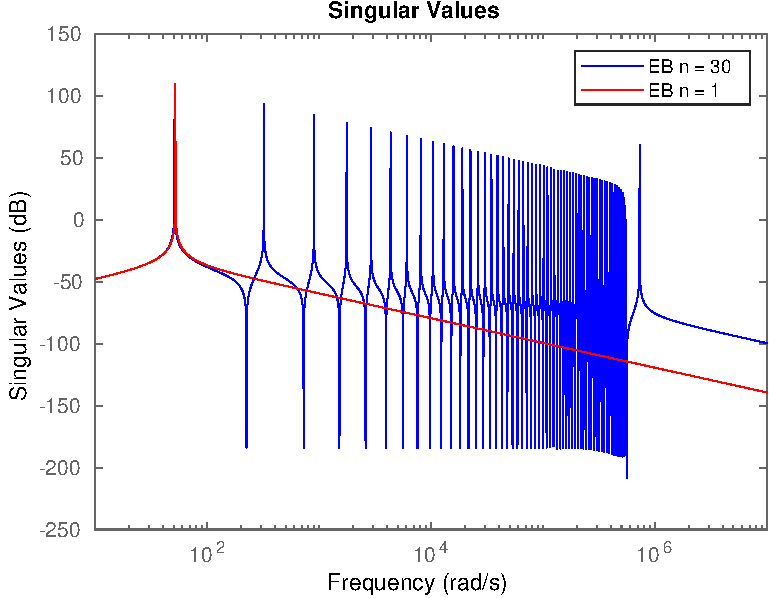
\includegraphics[width=0.32\textwidth]{Reduction/Reduction1.pdf} 
	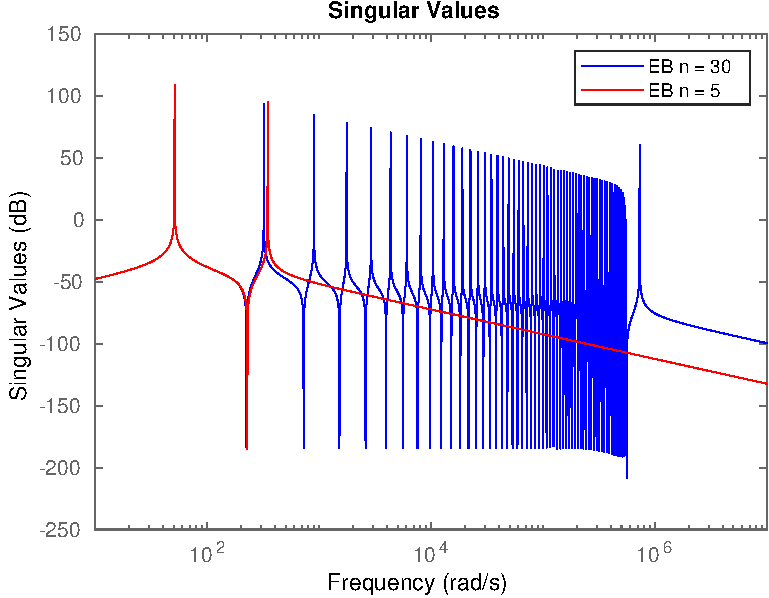
\includegraphics[width=0.32\textwidth]{Reduction/Reduction2.pdf}
	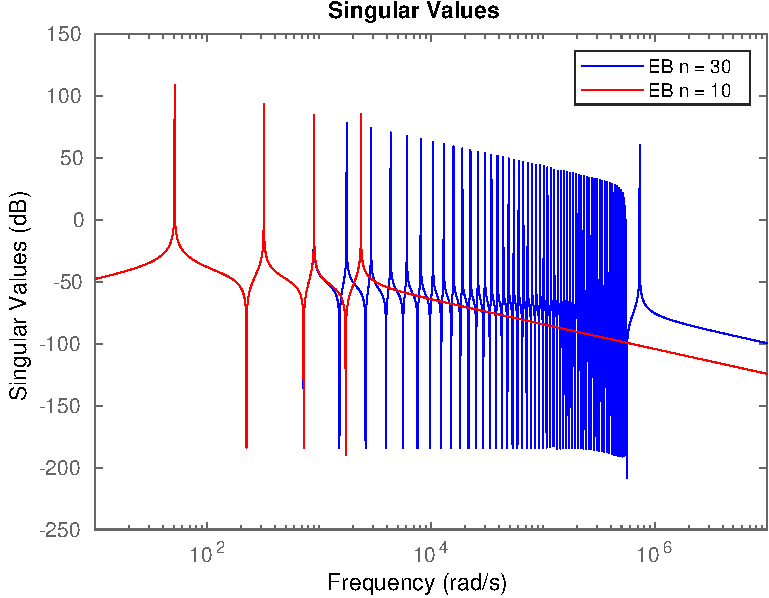
\includegraphics[width=0.32\textwidth]{Reduction/Reduction3.pdf}
	\caption{Krilov method\footfullcite{phdae_red} applied to the Euler Bernoulli beam}
\end{figure}

}
\end{frame}

\section{Applications}

\subsection{Kirchhoff plate}
\begin{frame}{Boundary stabilization of the Kirchhoff plate}
	\only<1>{Consider the problem
	\begin{equation*}\small
	\begin{bmatrix}
	\rho h & 0 \\ 0 & \mathbb{D}^{-1} \\
	\end{bmatrix}
	\diffp{}{t}
	\begin{bmatrix}
	w_t \\ \Sigma \\
	\end{bmatrix} = 
	\begin{bmatrix}
	0 & -\div\Div \\ \Grad\grad & 0 \\
	\end{bmatrix}
	\begin{bmatrix}
	w_t \\ \Sigma \\
	\end{bmatrix} \quad (x, y) \in \Omega = [0, 1]\times[0,1]
	\end{equation*}
	Boundary conditions
	\begin{align*}
		\begin{aligned}
		w_t|\Gamma_D &= 0, \\
		\partial_x w_t|\Gamma_D &= 0, \\
		\end{aligned} \qquad  \Gamma_D &= \left\{x = 0 \right\}\\
		\begin{aligned}
		\Sigma \cddot (n \otimes n)|\Gamma_N &= u_M, \; \\
		\mathcal{D} \Sigma|\Gamma_N := \widetilde{q}|\Gamma_N &= u_F,\\
		\end{aligned} \qquad \Gamma_N &= \left\{x = 0,\, x=1,\, y=1 \right\}
	\end{align*}

	with initial conditions (compatible with the constraints):
	\[
	w_t(x,y,0) = x^2; \qquad \Sigma(x,y,0) ={0}.
	\]
	}
	\only<2>{ Obtain a finite-dimensional uncontrolled system
	\begin{equation*}
	\begin{aligned}
	\begin{bmatrix}
	{M} & {0} \\
	{0} & {0} \\
	\end{bmatrix}\frac{d}{d t}
	\begin{pmatrix}
	{e}\\
	{\lambda} \\
	\end{pmatrix}
	&= \begin{bmatrix}
	{J} & {G} \\
	-{G}^T & {0} \\
	\end{bmatrix}
	\begin{pmatrix}
	{e} \\
	{\lambda} \\
	\end{pmatrix} + \begin{bmatrix}
	{B} \\
	0 \\
	\end{bmatrix} {u}, \\
	{y} &= \begin{bmatrix}
	{B}^T & {0} \\
	\end{bmatrix} \begin{pmatrix}
	{e}\\
	{\lambda} \\
	\end{pmatrix},
	\end{aligned} 
	\end{equation*}
Apply the control law $u = -Ky, \ K>0$
\begin{equation*}
\begin{bmatrix}
M & {0} \\
{0} & {0} \\
\end{bmatrix}
\frac{d}{d t}
\begin{pmatrix}
{e}\\
{\lambda} \\
\end{pmatrix}
= \begin{bmatrix}
{J} - {R} & {G} \\
-{G}^T & {0} \\
\end{bmatrix}
\begin{pmatrix}
e\\
{\lambda} \\
\end{pmatrix},
\end{equation*}
with ${R} = {B} {K} {B}^T \succeq 0$. \\
The Hamiltonian $\dot{H} = - e^T R e \le 0$ is a non increasing function and by La~Salle principle the equilibrium point $e = 0$ is asymptotically stable.	
	}

	
	\begin{center}
		\only<3>{
			\movie[width=0.42\textwidth, height = 0.7 \textheight]{Damping Kirchhoff Plate}{Videos/Kirchh_Damped_4faster.mp4}			
		}
		\only<4>{
			\includegraphics[height=0.9\textheight]{DampingInjection/HamiltonianDamped_cropped.eps}
		}
	\end{center}
\end{frame}

\begin{frame}{Boundary interconnection of the Kirchhoff plate}
The system is composed by a cantilever plate connected to a rigid rod. The interconnection is given by a compact operator.
\begin{equation*}
\small \text{dpH} \left\{ 
\begin{aligned}
\diffp{x_1}{t} &= \mathcal{J} \diffd{H_1}{x_1} \\
u_{\partial, 1}  &= \mathcal{B} \diffd{H_1}{x_1} \\
y_{\partial, 1} &= \mathcal{C} \diffd{H_1}{x_1} 
\end{aligned}
\right. \qquad
\text{pH} \left\{ 
\begin{aligned}
\diff{{x}_2}{t} &= {J} \diffp{H_2}{{x}_2} + {B} {u}_2 \\
{y}_{2} &= {B}^T \diffp{H_2}{{x}_2} + {D} {u}_2 \\
\end{aligned}, \qquad 
\right. 
\end{equation*} %

where $x_1 \in \mathscr{X}$,  $u_{\partial, 1}  \in \mathscr{U}, \, y_{\partial, 1} \in  \mathscr{Y} = \mathscr{U}^\prime$ belong to some Hilbert spaces (the prime denotes the topological dual of a space) and ${x}_2 \in \mathbb{R}^n, {u}, {y} \in \mathbb{R}^m$. The duality pairings for the boundary ports are denoted by
\[
\left\langle u_{\partial, 1}, \; y_{\partial, 1} \right\rangle_{\mathscr{U} \times \mathscr{Y}},  \qquad
\left\langle {u}_{2}, \; {y}_{2} \right\rangle_{\mathbb{R}^m}.
\]
For the interconnection, consider the compact operator $\mathcal{W}: \mathscr{Y} \rightarrow \mathbb{R}^m$ and the following power preserving interconnection
\begin{equation*}
\label{eq:int_inf}
{u}_2 = -\mathcal{W} \, y_{\partial, 1},  \qquad u_{\partial, 1} = \mathcal{W}^* \, {y}_2,
\end{equation*}
\end{frame}

\begin{frame}{Boundary interconnection of the Kirchhoff plate}
\begin{equation*}\small
\begin{aligned}
\text{Kirchhoff plate} \\
\begin{bmatrix}
\rho h & 0 \\ 0 & \mathbb{D}^{-1} \\
\end{bmatrix}
\diffp{}{t}
\begin{bmatrix}
w_t \\ \Sigma \\
\end{bmatrix} &= 
\begin{bmatrix}
0 & -\div\Div \\ \Grad\grad & 0 \\
\end{bmatrix}
\begin{bmatrix}
w_t \\ \Sigma \\
\end{bmatrix} \\
u_{\partial, \text{pl}} &= w_t(x = L_x, y), \\
y_{\partial, \text{pl}} &= \mathcal{D} \Sigma = \widetilde{q}_n(x = L_x, y).
\end{aligned} \qquad \qquad
\begin{aligned}
\text{Rigid rod} \\
\begin{bmatrix}
M & 0 \\
0   & J_G \\
\end{bmatrix} 
\displaystyle \diff{}{t}
\begin{pmatrix}
v_G \\ \omega_G \\
\end{pmatrix} & = \begin{pmatrix}
F_z \\ T_x \\
\end{pmatrix} = {u}_{\text{rod}}\vspace{1mm}, \\
{y}_{\text{rod}} &= \begin{pmatrix}
v_G \\ \omega_{G} \\
\end{pmatrix},
\end{aligned}
\end{equation*}
Space $\mathscr{Y}$ is the space of square-integrable functions on with support $\Gamma_{\text{int}} = \left\{ (x,y) \vert \; x=L_x, 0 \le y \le L_y  \right\}$. The compact interconnection operator then reads
\begin{equation*}
\mathcal{W} y_{\partial, \text{pl}} = \begin{pmatrix}
\int_{\Gamma_{\text{int}}} y_{\partial, \text{pl}} \d{s} \\
\int_{\Gamma_{\text{int}}} \left( y - L_y/2 \right) y_{\partial, \text{pl}} \d{s} \\
\end{pmatrix}.
\end{equation*}
The adjoint operator is then obtained considering that ${u}_{\text{rod}} = \mathcal{W} y_{\partial, \text{pl}}$ and that the inner product of $\mathbb{R}^m$ is easily converted to an inner product on the space $L^2(\Gamma_{\text{int}})$
\begin{align*}
\left\langle \mathcal{W} y_{\partial, \text{pl}}, \; {y}_{\text{rod}} \right\rangle_{\mathbb{R}^m} &= \left\langle y_{\partial, \text{pl}}, \, \mathcal{W}^* {y}_{\text{rod}}\right\rangle_{L^2(\Gamma_{\text{int}})}, \\
\mathcal{W}^* {y}_{\text{rod}} &= v_G + \omega_{G} \left( y - L_y/2 \right).
\end{align*}
\end{frame}


\begin{frame}{Results}
\begin{center}
\onslide*<1>{
\movie[width=0.42\textwidth, height = 0.7 \textheight]{Plate and rod}{Videos/Kirchh_Rod.mp4}	
\movie[width=0.42\textwidth, height = 0.7 \textheight]{Only plate}{Videos/Kirchh_NoRod.mp4}
}
\onslide*<2>{
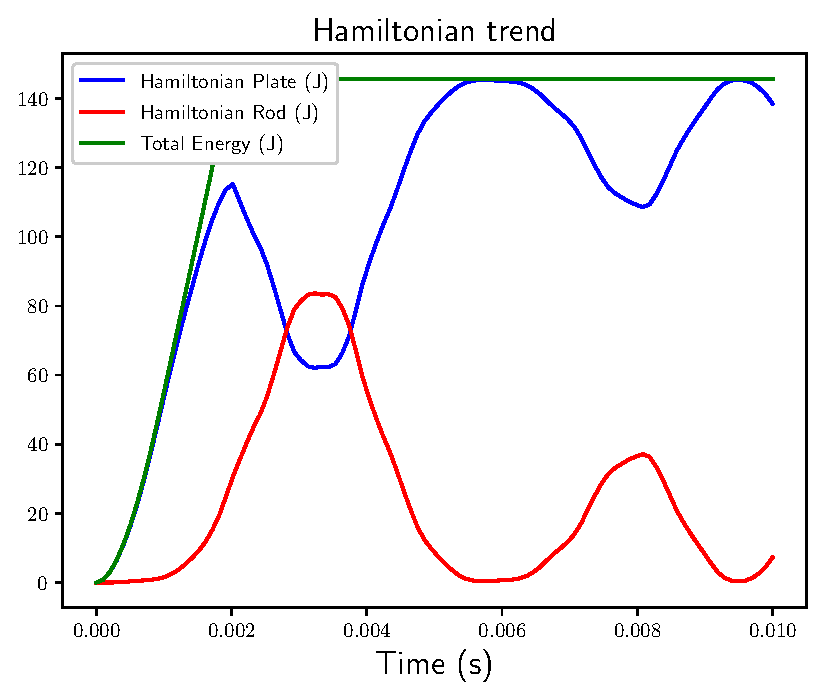
\includegraphics[width=0.42\textwidth]{InterconnectionRod/HamiltonianRod_cropped.eps}
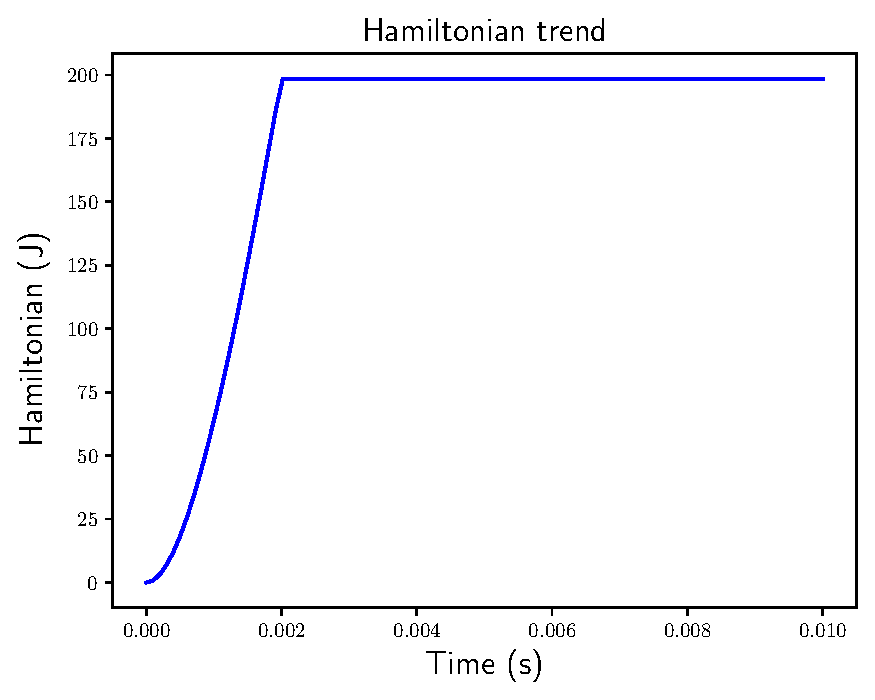
\includegraphics[width=0.44\textwidth]{InterconnectionRod/HamiltonianNoRod_cropped.eps}
}
\end{center}
\end{frame}

\subsection{Non linear Saint Venant}

\begin{frame}{Boundary stabilization of the Saint Venant model}
\only<1>{
	Consider the non linear system  PDE
	\begin{equation*}
	\diffp{}{t}\begin{bmatrix}
	h \\ \rho \bm{v}
	\end{bmatrix} = 
	\begin{bmatrix}
	0 & \div \\
	\grad & 0 \\
	\end{bmatrix}\begin{bmatrix}
	\rho g \left( h + \frac{1}{2}||\bm{v}||^2 \right) \\
	h \bm{v} \\
	\end{bmatrix} \qquad (x, y) \in \Omega = \left\{x^2 + y^2 \le  1\right\} 
	\end{equation*}
	With boundary condition 
	\[
	h \bm{v} \cdot \bm{n}|_{\partial \Omega} = u_\partial 
	\]
	This model represents the oscillations of waves in a reservoir with $h$ the fluid height and $\bm{v}$ the velocity field, with mass flux controlled on the boundary. 
}
\only<2>{The Hamiltonian
	\[ H = \frac{1}{2} \int_{\Omega}\rho g h^2 + \rho h ||\bm{v}||^2 \ \d{\Omega}
	\]
	is non separable $H \ne E(\bm{v}) + V(h)$. \\
	Selecting as energy variables $x_1 = h, \, \bm{x}_2 = \rho \bm{v}$, we get the pH system
	\begin{equation*}
	\diffp{}{t}\begin{bmatrix}
	x_1 \\ \bm{x}_2 \\
	\end{bmatrix} = 
	\begin{bmatrix}
	0 & \div \\
	\grad & 0 \\
	\end{bmatrix}\begin{bmatrix}
	\delta_{x_1} H\\
	\delta_{x_2} H\\
	\end{bmatrix}
	\end{equation*}
	With boundary condition 
	\[
	\delta_{x_1} H \cdot n|_{\partial \Omega}:= \rho h \bm{v} \cdot {n}|_{\partial \Omega} = u_\partial 
	\]
}
\only<3>{
	Considering as conjugated output the pressure $y_\partial = p = \rho g \left( h + \frac{1}{2}||\bm{v}||^2 \right)$ and using the control law 
	\[u_\partial = - k (y_\partial - y_\partial^0)
	\]
	with $y_\partial^0 = \rho g h_{\text{des}}$ the desired pressure at equilibrium. \\
	It can be shown that the Lyapunov function
	\[
	V = \frac{1}{2} \int_{\Omega} \rho g (h - h_{\text{des}})^2 + \rho h ||\bm{v}||^2 \d{\Omega},
	\]
	is non increasing 
	\[
	\dot{V} = - k \int_{\partial \Omega} (y_\partial - y_\partial^0)^2 \d{\Gamma} \le 0,
	\]
	and the equilibrium point $(h, \bm{v}) = (h_{\text{des}}, 0)$ is asymptotically stable.
}
\end{frame}

\begin{frame}{Results}
\begin{center}
	\onslide*<1>{
		Initial condition
		\[h(r, \theta, 0) = h_{\text{des}}(1 +  \cos(\pi r)  \cos(2 \theta)/10), \quad \rho \bm{v} = 0 \]
		\movie[width=0.42\textwidth, height = 0.7 \textheight]{Saint Venant in circular domain}{Videos/damped_saintvenant.mp4}
	}
	\onslide*<2>{
		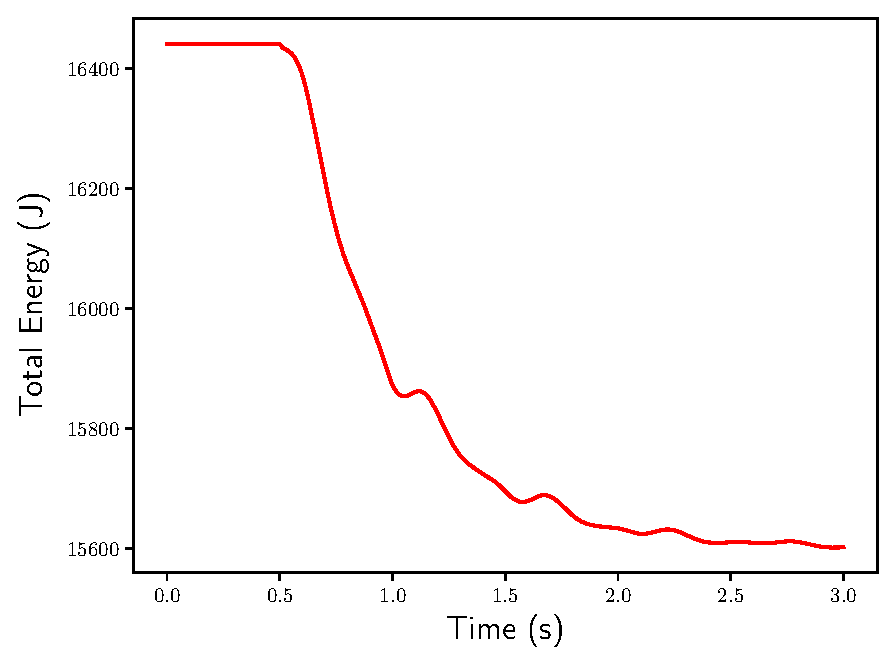
\includegraphics[width=0.44\textwidth]{SaintVenant/Hamiltonian.eps}
		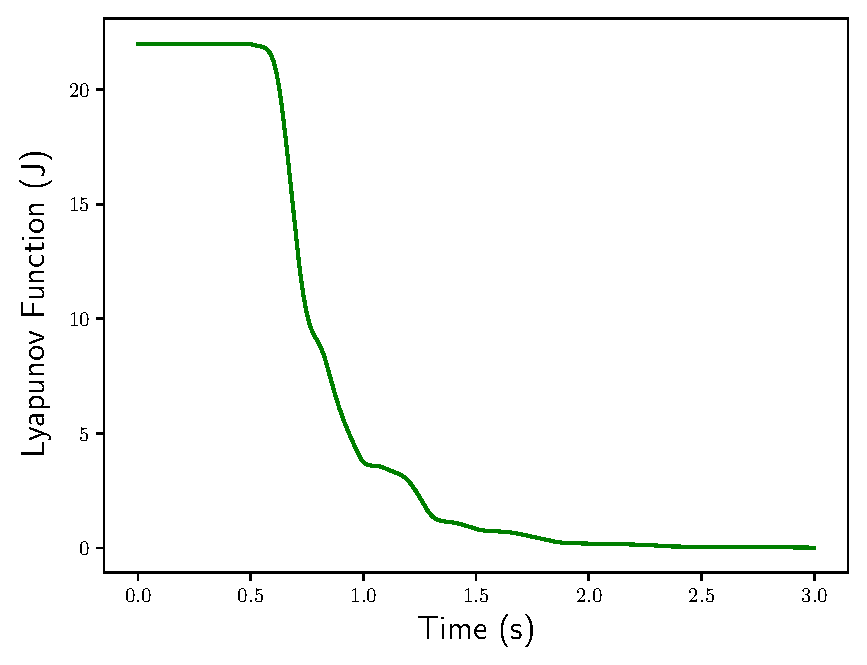
\includegraphics[width=0.44\textwidth]{SaintVenant/Lyapunov.eps}
	}
\end{center}
\end{frame}

\subsection{Vibroacoustic}

\begin{frame}{Dealing with mixed boundary control}
Propagation of acoustic waves in a cylindrical axis-symmetrical channel 
\begin{equation*}
\diffp{}{t}
\begin{bmatrix}
\chi_s p \\ \mu_0 \bm{v} \\
\end{bmatrix} = 
\begin{bmatrix}
0 & \div \\ \grad & 0 \\
\end{bmatrix}
\begin{bmatrix}
p \\ \bm{v} \\
\end{bmatrix}, \quad \Omega = \left\{x \in [0, L],\, r \in [0, R],\,  \theta \in [0, 2 \pi) \right\}
\end{equation*}
with a constant axial flow and an impedance conditions on the lateral surface. \\ 
Two discretization methods are compared: DAE with Lagrange multiplier and ODE with domain decomposition.\\

\centering
\includegraphics[height=0.3\textheight]{Vibroacoustic/domain_split.eps}
\end{frame}

\begin{frame}{Results}
\begin{center}
		\movie[width=0.42\textwidth, height = 0.7 \textheight]{Vibroacoustic DAE}{Videos/wave_dae10.mp4}
		\movie[width=0.42\textwidth, height = 0.7 \textheight]{Vibroacoustic ODE}{Videos/wave_ode10.mp4}
\end{center}
\end{frame}


\begin{frame}{Future developments}
\begin{itemize}
	\item Flexible multibody dynamics;
	\item Thermoelasticity?
\end{itemize}
\end{frame}

\begin{frame}{Thank you}
\centering
\Huge Questions
\end{frame}

\begin{frame}[allowframebreaks]{References}
\printbibliography
\nocite{*}
\end{frame}

\end{document}
